\section{Chapter 1: Introduction}
Mathematical models called ''machines.''
Collection of successful inputs are called the language of the machines.

\subsection{History}
\begin{itemize}
    \item Cantor (1845-1918) - Theory of sets (union, intersections, cardinality, etc) Discovered paradoxes such as the idea that infinity comes in different sizes, some set is bigger than the universal set.
    \item Hilbert (1906-1978) Methodology for finding proofs.
    Each true proposition is provided with a rigorous proof in which every line is either an axiom or follows from the axioms and previously proved theorems by a specified small set of rules of inference.
    \item Godel (1906-1978) Incompleteness theorem.
    There was no algorithm to provide proofs for all true statements in mathematics.
    He showed that either there were some true statements in mathematics that had no proofs, or else there were some false statements that did have proofs.
    \item Church, Kleene, Post, Markov, von Neumann, Turing - Which statements have proofs?
    Building blocks of mathematical algorithms.
    Turing proved that there were mathematically definable fundamental questions about the machine itself that the machine could not answer.
\end{itemize}

\subsection{Languages and Machines}
% p. 434
\begin{figure}[!ht]
    \centering
    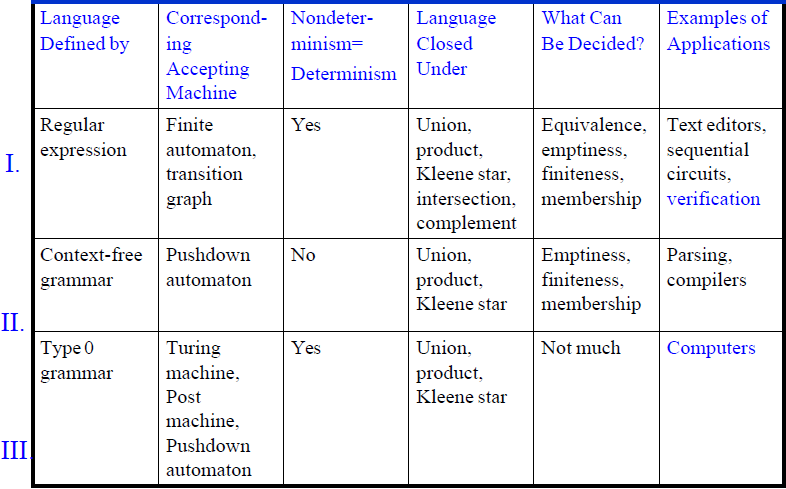
\includegraphics[width=\linewidth]{lecture 1/figures/page434.png}
    \caption{Page 434 in textbook.}
\end{figure}
The term computer is never used in this course. We study computers by building mathematical models called \textbf{machines}, and then studying their limitations by analyzing the types of inputs on which they operate successfully. The collection of successful inputs is called the \textbf{language} of the machine.